\documentclass[11pt]{article}

\usepackage[margin=1in]{geometry}
\usepackage{amsfonts}
\usepackage{amsmath}
\usepackage{graphicx}
\usepackage{algorithm}
\usepackage[noend]{algpseudocode}
\usepackage{url}
\usepackage{multirow}
\usepackage{authblk}
\usepackage{rotating}
\usepackage{xr}
\externaldocument[S]{nm_supp}

\usepackage[style=nature,maxbibnames=5,mincitenames=1,maxcitenames=1]{biblatex}
\renewbibmacro{in:}{%
  \ifentrytype{article}{}{%
  \printtext{\bibstring{in}\intitlepunct}}}
\addbibresource{nm.bib}

\newcommand{\degree}{\ensuremath{^\circ}}

\begin{document}

%\title{Cloudbreak: A MapReduce Algorithm for Detecting Genomic Structural Variation}
\title{Fast, Accurate, and Scalable Genomic Structural Variation Detection on the Cloud: MapReduce based {\em Cloudbreak}}

\author[1,5]{Christopher W. Whelan \thanks{whelanch@ohsu.edu}}
\author[3,4]{Jeffrey Tyner}
\author[6]{Alberto L'Abbate}
\author[6]{Clelia Tiziana Storlazzi}
\author[4,5]{Lucia Carbone}
\author[1,2,5]{Kemal S\"onmez \thanks{sonmezk@ohsu.edu}}
\affil[1]{Institute on Development and Disability and Center for Spoken Language Understanding}
\affil[2]{Department of Medical Informatics \& Clinical Epidemiology}
\affil[3]{Program in Molecular and Cellular Biosciences}
\affil[4]{Behavioral Neuroscience Department}
\affil[5]{Oregon Health \& Science University, Portland, OR, USA}
\affil[6]{Department of Genetics and Microbiology, University of Bari, Bari, Italy}

\maketitle


 \begin{abstract}
The detection of genomic structural variations (SV) remains one of the the most difficult challenges in analyzing high-throughput sequencing data due to the uncertainty inherent in short-read sequencing data and the  scale of the data sets. The growing size and number of sequencing data sets have rendered SV detection, and high throughput sequencing analysis in general, a bona fide big data problem and led to intense interest in distributing computation to cloud or commodity servers. Meanwhile, MapReduce is becoming a standard framework for distributing processing across compute clusters and has convincingly demonstrated its effectiveness in offering scalable solutions to big data problems. We describe a novel conceptual framework for SV detection algorithms in MapReduce based on computing local features along the genome. In this framework, we develop and evaluate a distributed deletion and insertion detection algorithm based on fitting a Gaussian mixture model to the distribution of mapped insert sizes spanning each location in the genome. On simulated and real data sets, our approach achieves performances meeting or exceeding those of a variety of popular structural variation detection algorithms, including read-pair, split-read, and hybrid approaches, and performs well across a wide range of deletion sizes. In particular, our algorithm excels at discovering insertions and deletions of size 40bp-100bp. In addition, our algorithm can accurately genotype heterozygous and homozygous deletions from diploid samples. Finally, our software offers dramatically faster runtimes than existing tools, given a sufficiently sized compute cluster, and also includes an automatic method to set up and configure MapReduce (Hadoop) clusters on a variety of cloud services, making cluster computing accessible to users who may not have the resources to maintain a MapReduce capable distributed compute server. Our implementation and source code are available at \url{http://github.com/cwhelan/cloudbreak}. 

 \medskip
 \noindent\textbf{Keywords:} genomic structural variation; distributed computing; copy number variation; high-throughput sequencing; genotyping.
 \end{abstract}


\newpage

\section{Introduction}

Genomic structural variations such as deletions, insertions, and inversions of DNA are widely prevalent in human populations and account for the majority of the bases that differ among normal human genomes \autocite{Mills:2011p1611, Conrad:2010ja}. However, detection of structural variations with current high-throughput sequencing technology remains a difficult problem, with limited concordance between available algorithms and high false discovery rates \autocite{Mills:2011p1611}.

Popular SV detection algorithms use three main signals present in high-throughput sequencing data sets. See \textcite{Alkan:2011p547} for a review. Read-pair (RP) based methods use the distance between and orientation of the mappings of the sequenced ends of DNA fragments to identify the signatures of SVs \autocite{Campbell:2008p539,Chen:2009p3,Hormozdiari:2009p284,Sindi:2009gu,Korbel:2009dy}. Traditionally, this involves separating mappings into those that are \emph{concordant} or \emph{discordant}, where discordant mappings deviate from the expected insert size or orientation of the fragment. These approaches then cluster the discordant mappings to find SVs with support from multiple discordantly mapped read pairs. Read-depth (RD) approaches, in contrast, consider the changing depth of coverage of concordantly mapped reads along the genome to infer the presence of SVs \autocite{Abyzov:2011bk,Alkan:2009cr,Yoon:2009kb,Chiang:2009di}. Finally, split-read (SR) methods look for breakpoints within individual reads by mapping portions of the read to different genomic locations \autocite{Wang:2011p1607,Ye:2009p2}.

The first RP methods used only unambiguously discordantly mapped read pairs in their analyses. However, it has been recently demonstrated that including multiple mappings of discordant read pairs in the analysis can improve sensitivity in repetitive regions of the genome \autocite{Hormozdiari:2009p284,Quinlan:2010gf}. More recently, several RP approaches have considered concordant read pairs, either to integrate RD signals for improved sensitivity and specificity \autocite{Sindi:2012kk,Michaelson:2012fj,Chiara:2012ey}, or to eliminate the thresholds necessary to separate concordant from discordant mappings and thus be able to detect smaller events \autocite{Marschall:2012ek}. Increasing the number of read mappings considered, however, increases the computational burden of SV detection. As large-scale sequencing projects and clinical sequencing applications emerge, fast runtimes and efficient storage of data are becoming increasingly important, although they have not been a focus of SV detection algorithm development.

Google's MapReduce \autocite{Dean:2008p277} framework was designed to manage the storage and efficient processing of very large scale data sets across clusters of commodity servers. Hadoop is an open source project of the Apache Foundation which provides an implementation of the MapReduce programming framework as well as a distributed file system (HDFS) for distributing the redundant storage of large data sets across a cluster. Use of the Hadoop framework has been demonstrated for several sequencing-related bioinformatic tasks including short read mapping \autocite{Schatz:2009p278}, SNP calling \autocite{Langmead:2009p1225}, and RNA-seq differential expression analysis \autocite{Langmead:2010p1268}.

Hadoop/MapReduce requires a specific programming model, however, which can make it difficult to design general-purpose algorithms for arbitrary sequencing analysis problems like SV detection. MapReduce divides computation across a cluster into three phases. In the first phase, \emph{mappers} developed by the application programmer examine small blocks of data and emit a set of $\langle key, value \rangle$ pairs for each block examined. The MapReduce framework then sorts the output of the mappers by key, and aggregates all values that are associated with each key. Finally, the framework executes \emph{reducers}, also created by the application developer, which process all of the values for a particular key and produce one or more outputs that summarize or aggregate those values. MapReduce and Hadoop allow efficient processing of large data sets by scheduling tasks for execution as close as possible to the nodes which hold the required data, minimizing network traffic and I/O contention.

The need to separate logic into mappers and reducers makes it difficult to implement traditional RP-based SV detection approaches in MapReduce, particularly given the global clustering of paired end mappings at the heart of many RP approaches. MapReduce algorithms, by contrast, excel at conducting many independent calculations in parallel. In sequencing applications, for example, MapReduce based SNP-callers Crossbow \autocite{Langmead:2009p1225} and GATK \autocite{McKenna:2010p1051} perform independent calculations for each location or partition in the genome. SV approaches that are similarly based on local computations have been described: the RP-based SV callers MoDIL \autocite{Lee:2009da} and forestSV \autocite{Michaelson:2012fj} attempt to solve the SV detection problem by computing scores or features along the genome and then producing SV predictions from those features in a post-processing step. 

In this paper, we describe a framework for solving SV detection problems in Hadoop and MapReduce based on the computation of local features along the genome from paired end mappings. We then demonstrate the development in this framework of a software package, Cloudbreak, for discovering genomic deletions up to 25,000bp long, and short insertions. Cloudbreak computes local features that build on the ideas implemented in MoDIL \autocite{Lee:2009da}, which modeled the distribution of insert sizes at each genomic location as a Gaussian Mixture Model (GMM). Use of the Hadoop/MapReduce framework enables scalable implementations of this class of algorithm. We characterize our algorithm's performance on simulated and real data sets and compare it with those of recently published methods.

\section{Results}

\subsection{Cloudbreak: A Hadoop/MapReduce Software Package for SV Detection}

\begin{figure}
\centering
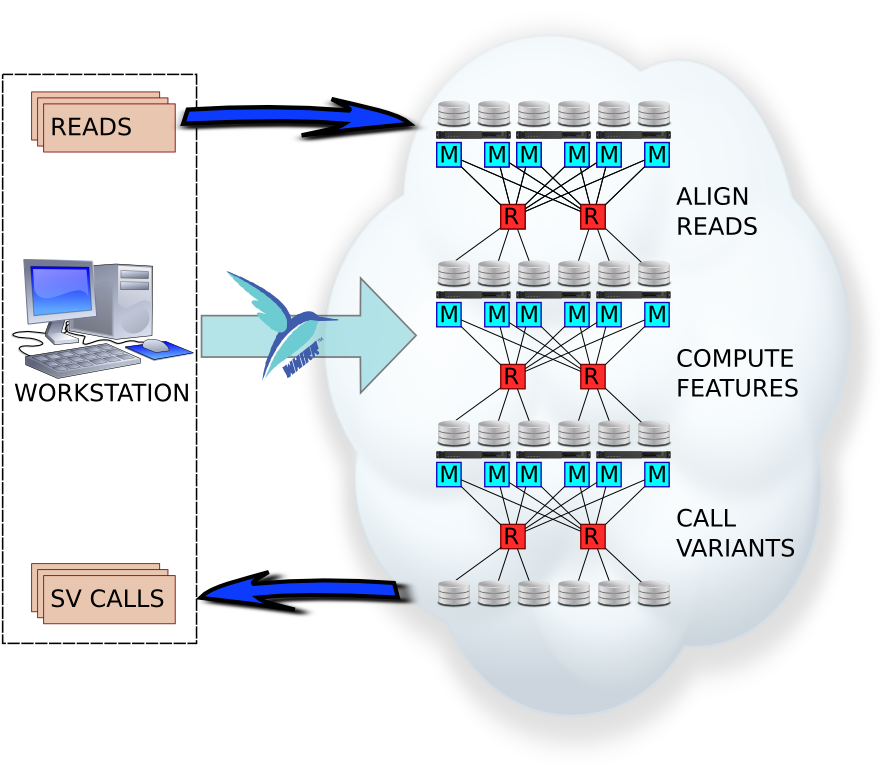
\includegraphics[width=.8\textwidth]{../figures/workflow_with_whirr.png}
\caption{An overview of the Cloudbreak workflow. Reads are first uploaded to a Hadoop cluster from local storage. Cloudbreak then executes three MapReduce jobs to process the data: 1) Mapping with sensitive settings. 2) Computation of features across the genome. 3) Calling structural variations based on the features computed in the previous step. Finally, SV predictions can be downloaded from the Hadoop cluster and examined. Cloudbreak can also use the Apache Whirr library to automatically provision Hadoop clusters on and deploy data to cloud providers such as Amazon Elastic Compute Cloud.}
\label{cloudbreak_workflow}
\end{figure}

Our framework for SV detection in MapReduce divides processing into three distinct MapReduce jobs. This framework is summarized in Figure \ref{cloudbreak_workflow}. Details of the MapReduce SV detection algorithmic framework and how Cloudbreak is implemented within that framework are provided in Supplementary Algorithm \ref{Scb_algo} and the Supplementary Materials; here we proceed with a high-level description of each job.

Cloudbreak's alignment job can run a variety of alignment tools that report reads in SAM format (Supplementary Materials). In the map phase, mappers align reads in either single-end or paired-end mode to the reference genome in parallel, outputting each possible mapping location as a value under a key identifying the read pair. In the reduce phase, the framework combines the reported mapping locations for the two ends of each read pair. 

In the next job, Cloudbreak computes a set of features for each location in the genome. To begin, we tile the genome with small fixed-width, non-overlapping windows. For the experiments reported in this paper we use a window size of 25bp. Within each window, we examine the distribution of insert sizes of read pairs that span that window, and compute features by fitting a Gaussian Mixture Model to that distribution (Supplementary Materials, Supplementary Figure \ref{Sinsert_size_mixes}). To remove incorrect mappings, we use an adaptive quality cutoff for each genomic location and then perform an outlier-detection based noise reduction technique (Supplementary Materials); these procedures also allow us to process multiple mappings for each read if they are reported by the aligner.

Finally, the third MapReduce job is responsible for making SV calls based on the features computed at each genomic location. In this job, we search for contiguous blocks of genomic locations with similar features and merge them into individual insertion and deletion SV calls, employing noise reduction techniques to increase specificity (Supplementary Materials).  We parallelize this job in MapReduce by making calls for each chromosome in parallel, which we achieve by associating a location and its set of features to its chromosome in the map phase, and then making SV calls for one chromosome in each reduce task. An illustration of the Cloudbreak algorithm working on a simple example is shown in Supplementary Figure \ref{Salgorithm_example}.

Cloudbreak can be executed on any Hadoop cluster; Hadoop abstracts away the details of cluster configuration, making distributed applications portable. In addition, our Cloudbreak implementation can leverage the Apache Whirr library to automatically create clusters with cloud service providers such as the Amazon Elastic Compute Cloud (EC2). This enables on demand provisioning of Hadoop clusters which can then be terminated when processing is complete, eliminating the need to invest in a standing cluster and allowing a model in which users can scale their computational infrastructure as their need for it varies over time.

\subsection{Tests with Simulated Data}

We compared the performance of Cloudbreak for detecting deletions and insertions to a selection of popular tools: the RP method BreakDancer \autocite{Chen:2009p3}, GASVPro, an RP method that integrates RD signals and ambiguous mappings to increase sensitivity and specificity \autocite{Sindi:2012kk}, the SR method Pindel \autocite{Ye:2009p2}, and the hybrid RP-SR method DELLY \autocite{Rausch:2012he}. DELLY produces two sets of calls, one based solely on RP signals, and the other based on RP calls that could be supported by SR evidence. We refer to these sets of calls as DELLY-RP and DELLY-SR in the following results. We also attempted to evaluate MoDIL on the same data. All of these methods detect deletions; in addition BreakDancer, Pindel, and MoDIL are capable of detecting insertions. See Methods for details on how reads were aligned and each program was invoked. For all alignments we used BWA \autocite{Li:2009p836}, although in testing Cloudbreak we have found that the choice of aligner, number of possible mapping locations reported, and whether the reads were aligned in paired-end or single-ended mode can have a variety of effects on the output of the algorithm (Supplementary Figure \ref{Salignment_comparison}).

As has been observed elsewhere, there is no available test set of real Illumina sequencing data from a sample that has a complete annotation of structural variations from the reference. Therefore, testing with simulated data is important to fully characterize an algorithm's performance characteristics. On the other hand, it is important that the simulated data contain realistic SVs that follow patterns of SVs observed in real data. To address this, we took one of the most complete lists of SVs from a single sample available, the list of homozygous insertions and deletions from the genome of J. Craig Venter \autocite{Levy:2007fb}. Using these variants, we simulated a 30X read coverage data set for a diploid human Chromosome 2 with a mix of homozygous and heterozygous variants, with 100bp reads and a mean fragment size of 300bp (See Methods).

\begin{figure}
\centering
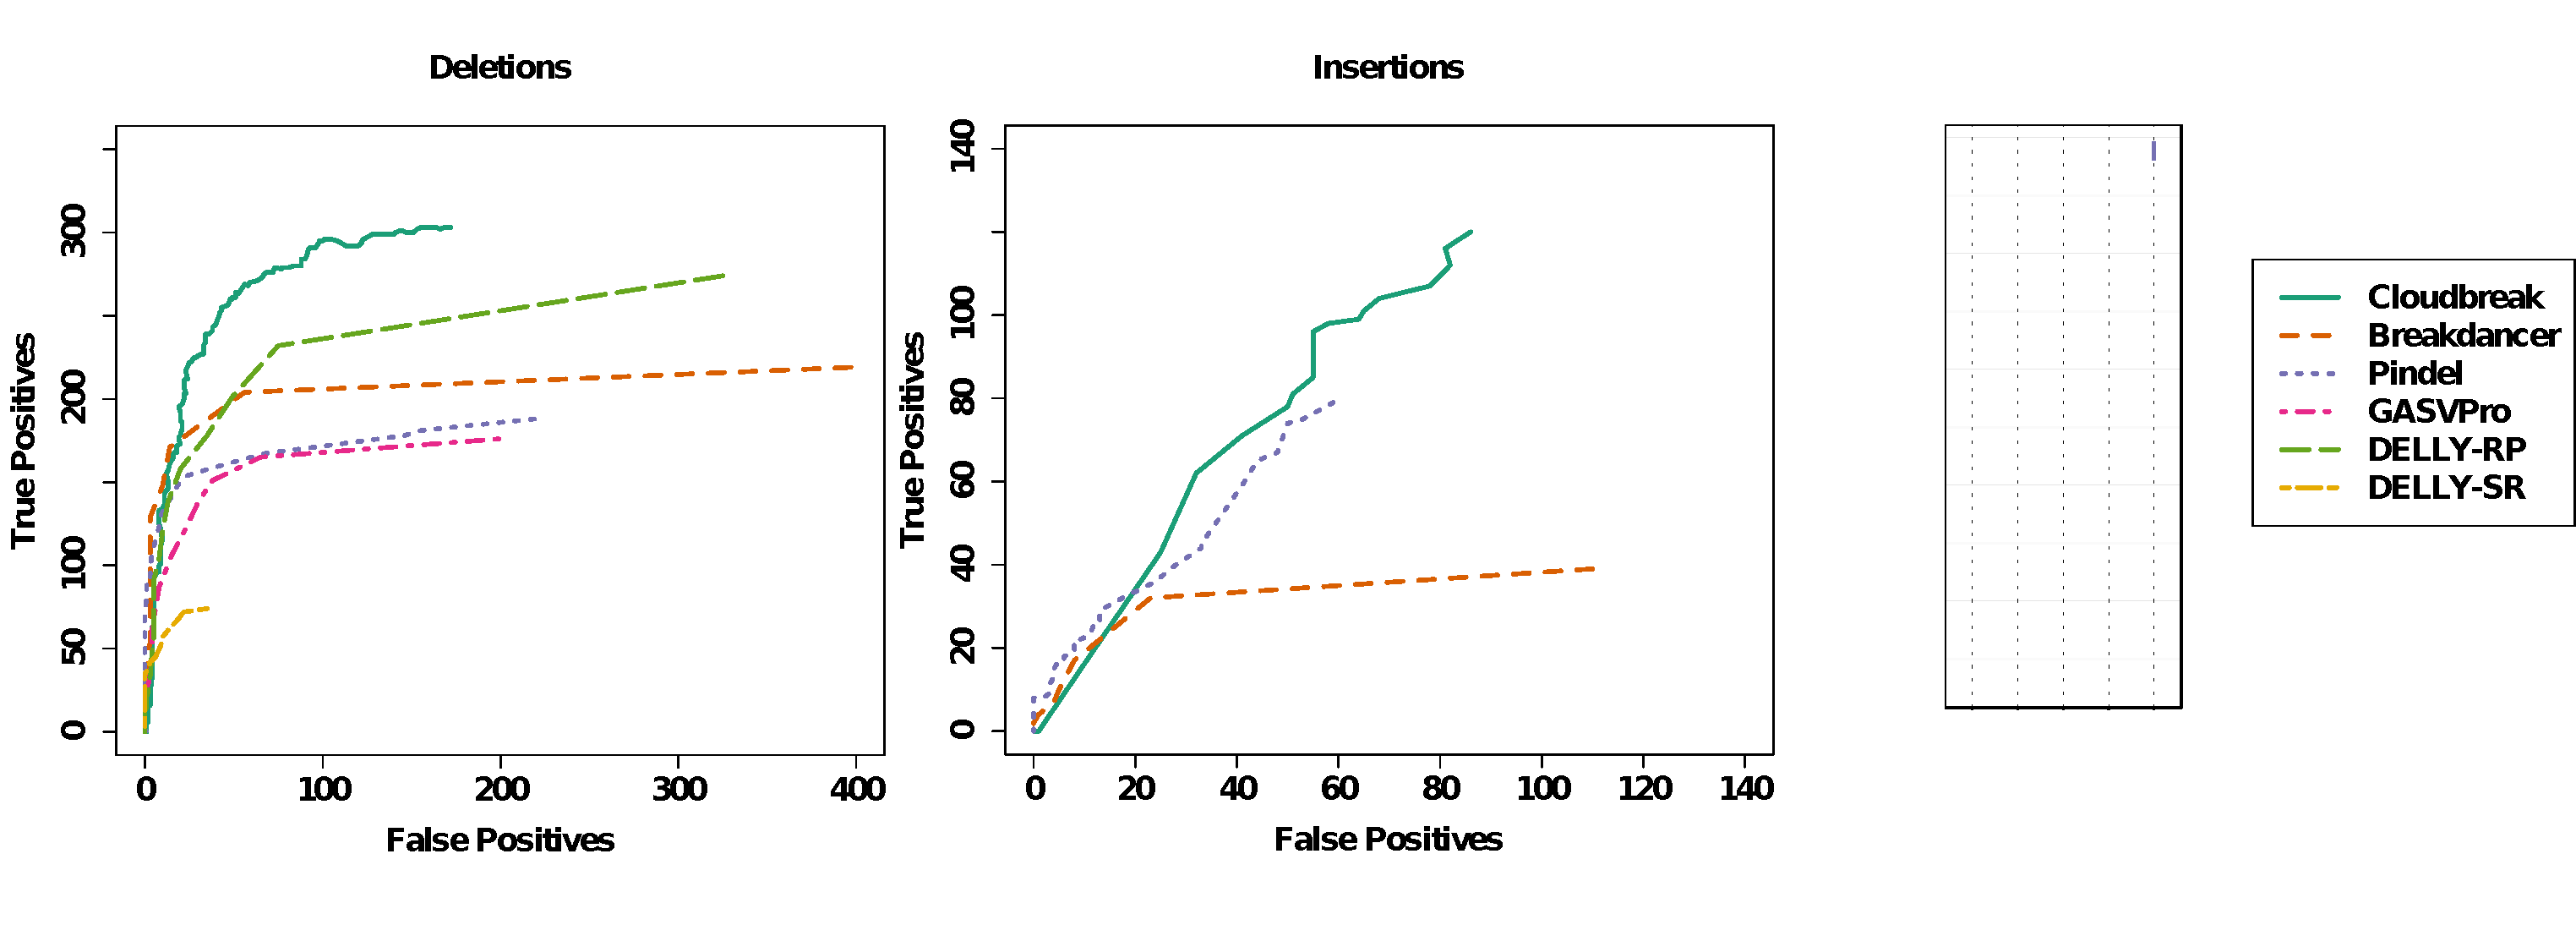
\includegraphics[width=1\textwidth]{../figures/chr2_sim_rocs_runtime.pdf}
\caption{Accuracy and runtime performance on a simulated data set. (a) Receiver Operating Characteristic (ROC) curves showing the specificity and sensitivity of each tool to deletions larger than 40bp on a simulated set of reads giving diploid coverage of 30X on human chromosome 2. Deletions from the Venter genome were randomly added to one or both haplotypes. Each point on a curve represents a different threshold on the confidence of predictions made by that tool. Thresholds vary by: Cloudbreak - likelihood ratio; BreakDancer, DELLY, GASVPro - number of supporting read pairs; Pindel - simple score. (b) ROC curves for insertion predictions. (c) Runtimes for each tool, not including alignment time, parallelized when possible (see Supplementary Material).}
\label{chr2CombinedRoc}
\end{figure}

Figure \ref{chr2CombinedRoc} shows Receiver Operating Characteristics (ROC) curves of the performance of each algorithm for detecting deletions and insertions on the simulated data set, as well as the runtimes of the approaches tested, excluding alignment. See Methods for a description of how we identified correct predictions. All approaches show excellent specificity at high thresholds in this simulation. Cloudbreak provides the greatest specificity for deletions at higher levels of sensitivity, followed by DELLY. For insertions, Cloudbreak clearly provides the best combinations of sensitivity and specificity. Cloudbreak's runtime is half that of BreakDancer, the next fastest tool, processing the simulated data in under six minutes. (Of course, Cloudbreak uses many more CPUs as distributed algorithm. See Supplementary Material and Supplementary Table \ref{Sruntimes} for a discussion of runtimes and parallelization.) The output which we obtained from MoDIL did not have a threshold that could be varied to correlate with the trade-off between precision and recall and therefore it is not included in ROC curves; in addition, MoDIL ran for 52,547 seconds using 250 CPUs in our cluster, so results are not included in the runtime figure. Apart from the alignment phase, which is embarrassingly parallel, the feature generation job is the most computationally intensive part of the Cloudbreak workflow. Therefore, to test scalability we measured the runtime of that job on Hadoop clusters made up of varying numbers of nodes and observed that linear speedups can be achieved in this portion of the algorithm by adding additional nodes to the cluster until a point of diminishing returns is reached (Supplementary Figure \ref{Sscalability}).

Choosing the correct operating point or threshold to set on the output of an SV calling algorithm can be difficult when operating on a new data set. The use of simulated data and ROC curves allows for some investigation of the performance characteristics of algorithms at varying levels. First, we characterized the predictions made by each algorithm at the operating point which gives them maximum sensitivity. For Cloudbreak we chose an operating point at which marginal improvements in sensitivity became very low. The results for both deletion and insertion predictions are summarized in Table \ref{chr2DeletionAndInsertionPredsMaxSensitivity}. MoDIL and Cloudbreak exhibited the greatest recall for deletions. Cloudbreak has high precision and recall for deletions at this threshold, and discovers many more small deletions. For insertions, Cloudbreak has the highest recall, although recall is low for all four approaches. Cloudbreak again identifies the most small variants. Pindel is the only tool which can consistently identify large insertions, as insertions larger than the library insert size do not produce mapping signatures detectable by read-pair mapping. We also used the ROC curves to attempt to characterize the predictions made by each algorithm when a low false discovery rate is required. Supplementary Table \ref{Schr2DeletionPredsFDR10} shows the total number of simulated deletions found by each tool when choosing a threshold that gives an FDR closest to 10\% based on the ROC curve. At this more stringent threshold, Cloudbreak identifies more deletions in every size category than any other tool. Performance on insertions never reached an FDR of 10\% for any threshold, so insertion predictions are not included in this table. We also examined Cloudbreak's ability to detect events in repetitive regions of the genome, and found that it was similar to the other methods tested (Supplementary Tables \ref{SdeletionRepmaskpreds} and \ref{SinsertionRepmaskpreds}).

It should be noted that the methods tested here vary in their breakpoint resolution (Supplementary Figure \ref{Sbreakpoint_resolution}): SR methods have higher resolution than RP methods. Cloudbreak sacrifices additional resolution by dividing the genome into 25bp windows; we strive however to increase sensitivity and specificity to actual variants in the hopes that such calls could still be useful even if their resolution is limited. This seems reasonable to us, especially given the possibility of pipelines in which RP calls are validated \emph{in silico} by local assembly methods or split-read methods.


\begin{table}[t]
\begin{center}
\resizebox{\textwidth}{!}{
\begin{tabular}{r|rrr|rrrrr}
  \cline{2-9}
   &                     & Prec. & Recall & 40-100bp  & 101-250bp  & 251-500bp & 501-1000bp & $>$ 1000bp \\ 
\hline
\multirow{7}{*}{\begin{sideways}Deletions\end{sideways}} & Total Number &          &           & 224 &  84 & 82 &  31 & 26\\ 
  \hline
\cline{2-9}
&  Cloudbreak    &  0.638 & \textbf{0.678} & \textbf{153} (9)  & 61 (0) &  62 (0) & 12 (0) & 15 (0) \\ 
&  BreakDancer   &  0.356 & 0.49 & 89 (0)  & 54 (0) &  53 (0) & 8 (0) & 15 (0) \\ 
&  GASVPro        & 0.146 & 0.432 & 83 (2)  & 32 (0) &  55 (0) & 8 (0) & 15 (0) \\ 
&  DELLY-RP           & 0.457 & 0.613 & 114 (3)  & \textbf{68} (0) &  \textbf{66} (0) & 9 (1) & 17 (0) \\ 
&  DELLY-SR           & \textbf{0.679} & 0.166 & 0 (0)  & 3 (0) &  49 (0) & 6 (0) & 16 (0) \\ 
&  Pindel           & 0.462 & 0.421 & 96 (\textbf{11})  & 24 (0) &  48 (0) & 5 (0) & 15 (0)\\ 
&  MoDIL           & 0.132  & 0.66 & 123 (6)  & 66 (\textbf{3}) &  \textbf{66} (\textbf{11}) & \textbf{17} (\textbf{7}) & \textbf{23} (\textbf{8})\\ 
   \hline
\multirow{5}{*}{\begin{sideways}Insertions\end{sideways}} & Total Number &          &           & 199 &  83 & 79 &  21 & 21\\ 
\cline{2-9}
&  Cloudbreak   &0.451 & \textbf{0.305}  & \textbf{79} (\textbf{32})  & \textbf{32} (\textbf{18}) &  \textbf{11} (8) & 1 (0) & 0 (0) \\ 
&  BreakDancer & 0.262 & 0.0968  & 23 (5)  & 14 (5) &  2 (1) & 0 (0) & 0 (0) \\ 
&  Pindel          & \textbf{0.572} & 0.196 & 52 (25)  & 5 (1) &  10 (\textbf{9}) & \textbf{3} (\textbf{2}) & \textbf{9} (\textbf{9})\\ 
&  MoDIL          & 0.186 & 0.0521 & 14 (1)  & 4 (0) &  1 (0) & 2 (\textbf{2}) & 0 (0)\\ 
\hline
\end{tabular}
}
\end{center}
\caption{The number of simulated deletions and insertions in the 30X diploid chromosome 2 with Venter indels found by each tool at maximum sensitivity, as well as the number of those variants that were discovered exclusively by each tool (in parentheses). The total number of variants in each size class in the true set of deletions and insertions is shown in the first row of each section.}
\label{chr2DeletionAndInsertionPredsMaxSensitivity}
\end{table}

\subsection{Tests with Biological Data}

We downloaded a data set of reads taken from a DNA sample of Yoruban individual NA18507, experiment ERX009609 from the Sequence Read Archive. This sample was sequenced on the Illumina Genome Analyzer II platform with 100bp paired end reads and a mean fragment size (minus adapters) of 300bp, with a standard deviation of 15bp, to a depth of approximately 37X coverage.

To create a gold standard set of insertions and deletions to test against, we pooled annotated variants discovered by three previous studies on the same sample. These included data from the Human Genome Structural Variation Project reported by \textcite{Kidd:2008p926}, a survey of small indels conducted by \textcite{Mills:2011fi}, and insertions and deletions from the merged call set of the phase 1 release of the 1000 Genomes Project \autocite{GenomesProjectConsortium:2012co} which were genotyped as present in NA18507. We merged any overlapping calls of the same type into the region spanned by their unions. It should be noted that the 1000 Genomes call set was partially produced using DELLY and BreakDancer, and therefore those calls are ones that those tools are sensitive to, biasing this test in their favor. We were unable to run MoDIL on the whole-genome data set due to the estimated runtime and storage requirements.

\begin{figure}
\centering
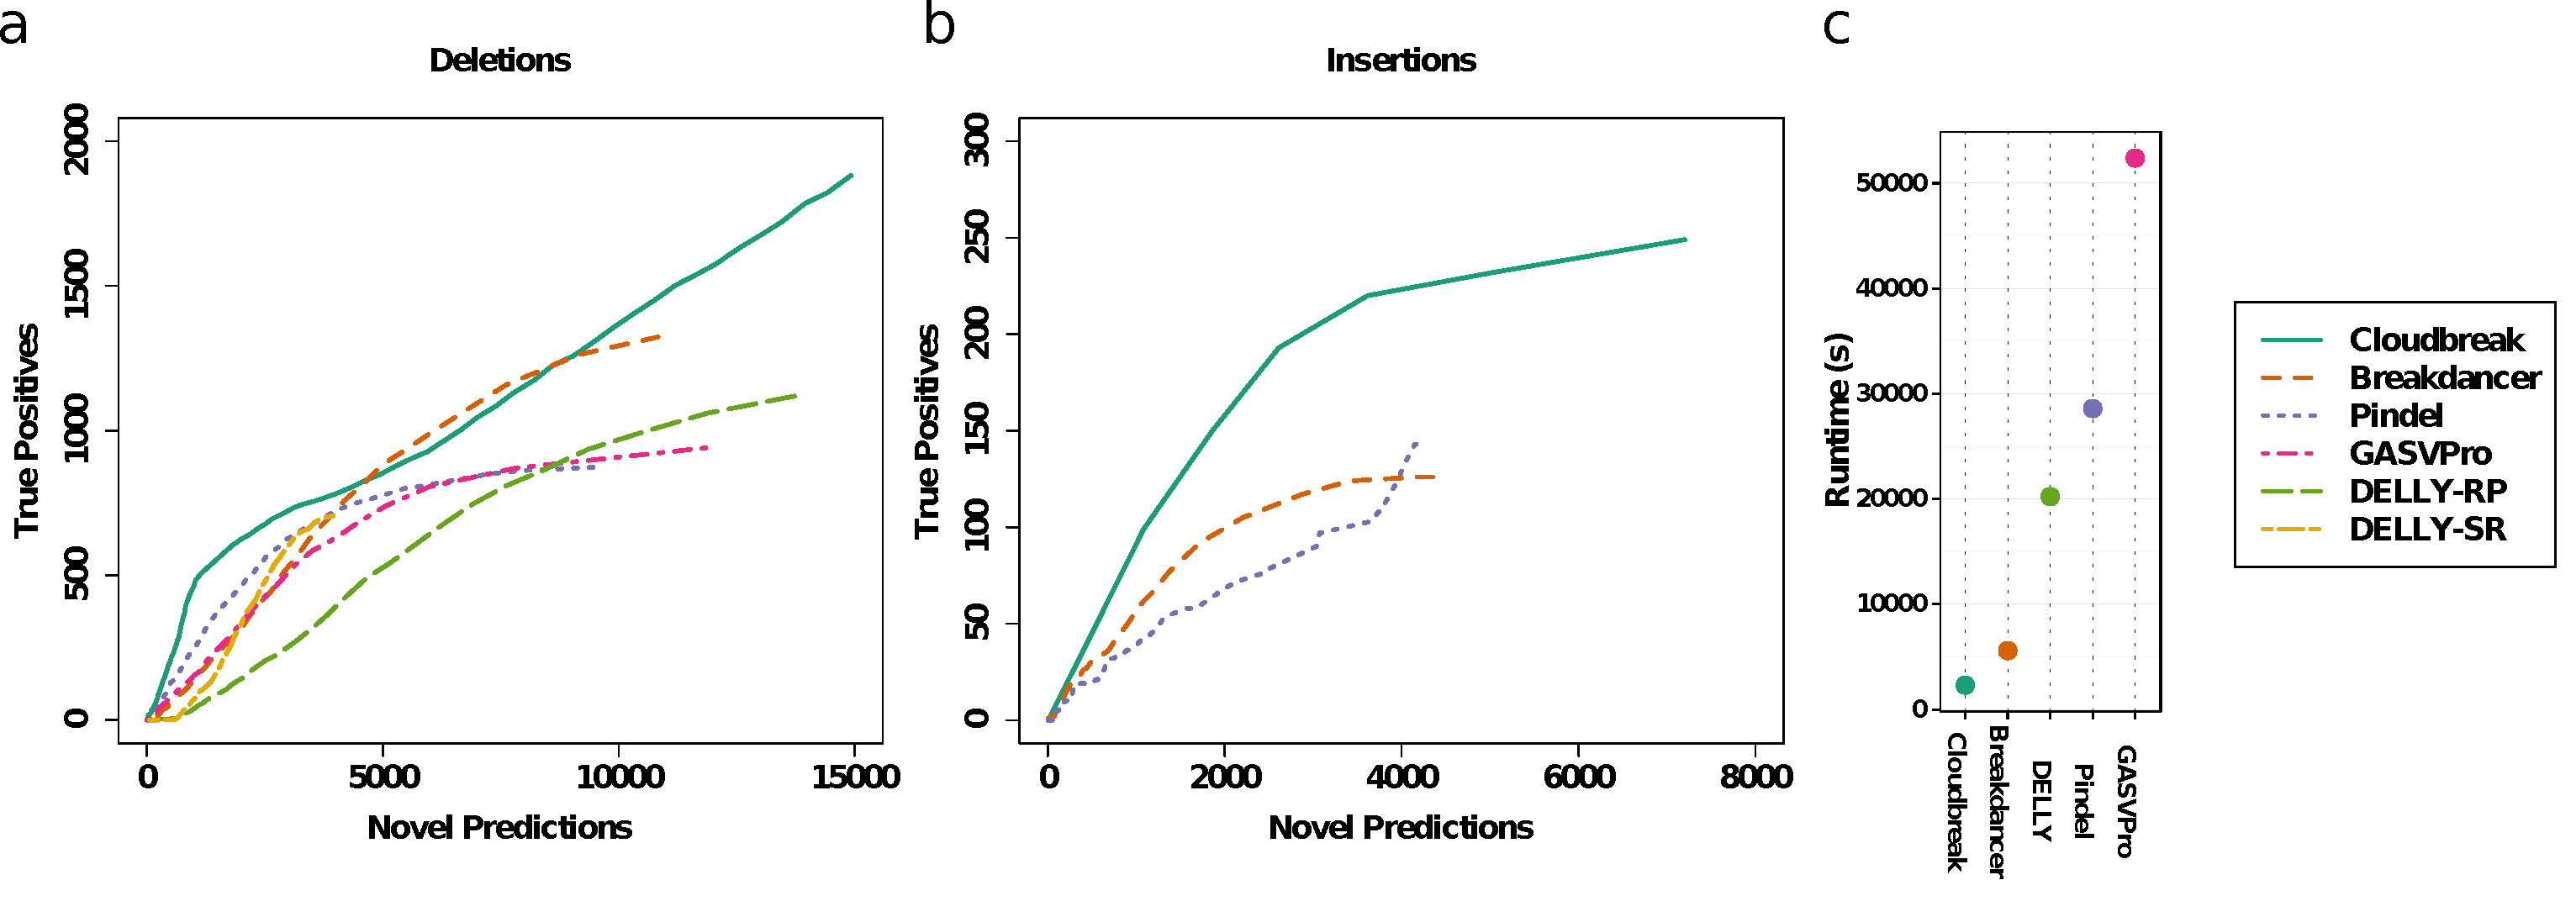
\includegraphics[width=1\textwidth]{../figures/NA18507_rocs_runtime.pdf}
\caption{Accuracy and performance on the 37X NA18507 sample. (a) ROC curve for deletion prediction performance, tested against the combined gold standard sets of deletions taken from \textcite{Kidd:2008p926}, \textcite{Mills:2011fi}, and \textcite{GenomesProjectConsortium:2012co}. (b) ROC curve for insertion prediction performance. (c) Runtimes for each tool, not including alignment time, parallelized when possible (see Supplementary Material). }
\label{NA18507CombinedRoc}
\end{figure}

Figure \ref{NA18507CombinedRoc} shows the performance of each algorithm on the NA18507 data set when compared against the gold standard set for both deletions and insertions. All algorithms show far less specificity for the gold standard set than they did for the true variants in the single chromosome simulation, although it is difficult to tell how much of the difference is due to the added complexity of real data and a whole genome, and how much is due to missing variants in the gold standard set that are actually present in the sample. For deletions, Cloudbreak is the best performer at the most stringent thresholds, and has the highest or second highest precision at higher sensitivity levels. Cloudbreak has slightly lower accuracy for insertions than other tools, although it can identify the most variants at higher levels of sensitivity. Cloudbreak processes the sample in under 15 minutes on our cluster, more than six times as fast as the next fastest program, BreakDancer, even when BreakDancer is run in parallel for each chromosome on different nodes in the cluster (see Methods and Supplementary Material).

Given the high number of false positives produced by all tools at maximum sensitivity indicated by the ROC curves, we decided to characterize the predictions made by each tool at more stringent thresholds. We examined the deletion predictions made by each algorithm using the same cutoffs that yielded a 10\% FDR on the simulated chromosome 2 data set, adjusted proportionally for the difference in coverage from 30X to 37X. For insertions, again, we were forced to use the thresholds that gave maximum sensitivity for each tool due to the high observed FDR rates in the simulated data. The precision and recall at these thresholds with respect to the gold standard set, as well as the performance of each algorithm at predicting variants of each size class at those thresholds, is shown in Table \ref{NA18507DeletionAndInsertionPreds}. For deletions, Cloudbreak has the greatest sensitivity of any tool at these thresholds, identifying the most variants in each size class. Pindel exhibits the highest precision with respect to the gold standard set. For insertions, Pindel again has the highest precision at maximum sensitivity, although according the ROC curve it is possible to choose a threshold for Cloudbreak with higher precision and recall. At maximum sensitivity, Cloudbreak identifies 120 more insertions from the gold standard set than Pindel, giving it by far the highest recall.

\begin{table}
\begin{center}
\resizebox{\textwidth}{!}{
\begin{tabular}{r|rrr|rrrrr}
  \cline{2-9}
&  & Prec. & Recall & 40-100bp & 101-250bp & 251-500bp & 501-1000bp & $>$ 1000bp \\ 
\hline
\multirow{6}{*}{\begin{sideways}Deletions\end{sideways}} & Total Number & & & 7,462 & 240 & 232 & 147 & 540 \\
  \hline
\cline{2-9}
& Cloudbreak & 0.0943 & \textbf{0.17} & \textbf{573} (\textbf{277})  & \textbf{176} (\textbf{30}) &  \textbf{197} (\textbf{18}) & \textbf{121} (\textbf{6}) & \textbf{399} (\textbf{24}) \\ 
& BreakDancer & 0.137 & 0.123 & 261 (29)  & 136 (3) &  178 (0) & 114 (0) & 371 (0) \\  
&  GASVPro & 0.147 & 0.0474 & 120 (21)  & 40 (2) &  85 (0) & 36 (0) & 128 (0) \\ 
&  DELLY-RP & 0.0931 & 0.1 & 143 (6)  & 128 (3) &  167 (1) & 103 (0) & 323 (1) \\ 
&  DELLY-SR & 0.153 & 0.0485 & 0 (0)  & 26 (0) &  123 (0) & 66 (0) & 203 (0) \\ 
&  Pindel & \textbf{0.179} & 0.0748 & 149 (8)  & 61 (0) &  149 (0) & 69 (1) & 217 (0) \\ 
\hline
\multirow{4}{*}{\begin{sideways}Insertions\end{sideways}} & Total Number & & & 536 & 114 & 45 & 1 & 0 \\
\cline{2-9}
& Cloudbreak & 0.0323 & \textbf{0.455} & \textbf{265} (\textbf{104})  & \textbf{49} (\textbf{24}) &  3 (1) & 0 (0)  & 0 (0)  \\ 
& BreakDancer & 0.0281 & 0.181 & 97 (10)  & 27 (5) &  2 (1) & 0 (0) & 0 (0) \\  
&  Pindel & \textbf{0.0387} & 0.239 & 144 (45)  & 14 (7) &  \textbf{7} (\textbf{6}) & \textbf{1} (\textbf{1}) &  0 (0) \\ 
\hline
\end{tabular}
}
\end{center}
\caption{The precision and recall with respect to the gold standard set of deletions and insertions for each tool on the NA18507 data, as well as the number of variants found in each size class found. Exclusive predictions are in parentheses. For deletions, the same cutoffs were used as for the simulated data as in Supplementary Table \ref{Schr2DeletionPredsFDR10}, adjusted for the difference in coverage from 30X to 37X. For insertions, the maximum sensitivity cutoff was used.}
\label{NA18507DeletionAndInsertionPreds}
\end{table}

\subsection{Performance on a Low-Coverage Cancer Data Set}

We also tested Cloudbreak on a sequencing data set obtained from a patient with acute myeloid leukemia (AML). This data set consisted of 76bp paired end reads with a mean insert size of 285bp and standard deviation of 50bp, yielding sequence coverage of 5X and physical coverage of 8X. Using a pipeline consisting of Novoalign, BreakDancer, and a set of custom scripts for filtering and annotating candidate SVs, we had previously identified a set of variants present in this sample and validated several using PCR, including 8 deletions. Cloudbreak was able to identify all 8 of the validated deletions, showing that it is still sensitive to variants even when using lower coverage data sets with a greater variance of insert sizes. The variants identified include deletions in the gene CTDSPL/RBPS3, an AML tumor suppressor \autocite{Zheng:2012kk}, and NBEAL1, a gene up-regulated in some cancers \autocite{Chen:2004jo}. We are currently investigating these deletions to determine their functional impact on this patient. 

\subsection{Genotyping Variants}

Because Cloudbreak explicitly models zygosity in its feature generation algorithm, it is possible to predict the genotypes of identified variants. We tested this on both the simulated and NA18507 data sets. Because we simulated a diploid genome, we had genotypes for the simulated data readily available. For the real dataset, we only considered the deletions from the 1000 Genomes Project data set, which had been genotyped as part of the Phase 1 release using the population-scale SV detection algorithm Genome STRiP \autocite{Handsaker:2011ki}. Cloudbreak was able to achieve 92.7\% and 95.9\% accuracy in predicting the genotype of the true positive deletions we detected at our 10\% FDR threshold in the simulated and real data sets, respectively. Supplementary Table \ref{SdeletionGenotypeaccuracy} shows confusion matrices for the two samples using this classifier. None of the three input sets that made up the gold standard for NA18507 contained a sufficient number of insertions that meet our size threshold that also had genotyping information. Of the 123 insertions detected by Cloudbreak on the simulated data set, 43 were heterozygous. Cloudbreak correctly classified 78 of the 80 homozygous insertions and 31 of the 43 heterozygous insertions discovered, for an overall accuracy rate of 88.6\%.

\section{Discussion}\label{Discussion}

Over the next few years, due to advances in sequencing technology, genomics data are expected to increase both in volume and in coverage by several orders of magnitude, expanding into the realm referred to as Big Data. In addition, the usage of existing information will increase drastically as research in genomics grows and translational applications are developed, and the data sets are reprocessed and integrated into new pipelines. In order to capitalize on this emerging wealth of genome data, novel computational solutions that are capable of scaling with the increasing number and size of these data sets will have to be developed. 

Among Big Data infrastructures, MapReduce is emerging as a standard framework for distributing computation across compute clusters. In this paper, we introduce a novel conceptual framework for structural variation detection algorithms in MapReduce, based on computing local features along the genome. This framework provides a scalable basis for developing SV detection algorithms, as demonstrated by our development of a distributed deletion-finding algorithm based on fitting a GMM to the distribution of mapped insert sizes spanning each location in the genome. 

On simulated and real data sets, our approach performs well across a wide range of deletion sizes and achieves performance similar to or better than a variety of state-of-the-art structural variation detection algorithms that run on traditional workload clusters and servers. Detection of deletions is an important area of research; \textcite{Mills:2011fi} recently identified over 220 coding deletions in a survey of a large number of individuals, and they note that such variants are likely to cause phenotypic variation in humans. In addition, an increased ability to detect variants in regions of the genome that are repetitive and difficult to align reads to opens up new possibilities in exploring human genetic variation.

In addition to delivering state-of-the-art performance in a RP-based SV detection problem, our approach offers a basis for developing a variety of SV algorithms that are capable of running in a MapReduce pipeline with the power to process vast amounts of data in a cloud or commodity server setting. Using tools like Apache Whirr (\texttt{http://whirr.apache.org/}, it is becoming trivially easy to instantiate on-demand Hadoop compute clusters with cloud providers such as Amazon's EC2. Having computational approaches that can harness this capability will become increasingly important for researchers or clinicians who are unable to afford or unwilling to maintain large, specialized servers to analyze their data.

\newpage

\section{Methods}\label{discussion}

\subsection{Cloudbreak Implementation}
Cloudbreak is a native Java Hadoop application. We deployed Cloudbreak on a 56-node cluster running the Cloudera CDH3 Hadoop distribution, version 0.20.2-cdh3u4. We use snappy compression for MapReduce data. Hadoop's distributed cache mechanism shares the executable files and indices needed for mapping tasks to the nodes in the cluster. To execute the other tools in parallel mode we wrote simple scripts to submit jobs to the cluster using the HTCondor scheduling engine (\url{http://research.cs.wisc.edu/htcondor/}) with directed acyclic graphs to describe dependencies between jobs. 

\subsection{Cloudbreak Genotyping}
We used the parameters of the fit GMM to infer the genotype of each predicted variant. Assuming that our pipeline is capturing all relevant read mappings near the locus of the variant, the genotype should be indicated by the estimated parameter $\alpha$, the mixing parameter that controls the weight of the two components in the GMM. We setting a simple cutoff of .35 on the average value of $\alpha$ for each prediction to call the predicted variant homozygous or heterozygous. We used the same cutoff for deletion and insertion predictions.

\subsection{Read Simulation}
Since there are relatively few heterozygous insertions and deletions annotated in the Venter genome, we used the set of homozygous indels contained in the HuRef data (\texttt{HuRef.homozygous\_indels.061109.gff}) and randomly assigned each variant to be either homozygous or heterozygous. Based on this genotype, we applied each variant to one or both of two copies of the human GRCh36 chromosome 2 reference sequence. We then simulated paired Illumina reads from these modified references using \emph{dwgsim} from the DNAA software package (\url{http://sourceforge.net/apps/mediawiki/dnaa/}). We simulated 100bp reads with a mean fragment size of 300bp and a standard deviation of 30bp, and generated 15X coverage for each modified sequence. Pooling the reads from both simulations gives 30X coverage for a diploid sample with a mix of homozygous and heterozygous insertions and deletions.

\subsection{Read Alignments}
Simulated reads were aligned to hg18 chromosome 2, and NA18507 reads were aligned to the hg19 assembly. Alignments for all programs, unless otherwise noted, were aligned using BWA \autocite{Li:2009p836} \texttt{aln} version 0.6.2-r126, with parameter \texttt{-e 5} to allow for longer gaps in alignments due to the number of small indels near the ends of larger indels in the Venter data set. GASVPro also accepts ambiguous mappings; we extracted read pairs that did not align concordantly with BWA and re-aligned them with Novoalign V2.08.01, with parameters \texttt{-a -r -Ex 1100 -t 250}. 

\subsection{SV Tool Execution}
We ran BreakDancer version 1.1\_2011\_02\_21 in single threaded mode by first executing \texttt{bam2cfg.pl} and then running \texttt{breakdancer\_max} with the default parameter values.  To run Breakdancer in parallel mode we first ran \texttt{bam2cfg.pl} and then launched parallel instances of \texttt{breakdancer\_max} for each chromosome using the \texttt{-o} parameter. We ran DELLY version 0.0.9 with the \texttt{-p} parameter and default values for other parameters. For the parallel run of DELLY we first split the original BAM file with BamTools \autocite{Barnett:2011hm}, and then ran instances of DELLY in parallel for each BAM file. We ran GASVPro version 1.2 using the \texttt{GASVPro.sh} script and default parameters. Pindel 0.2.4t was executed with default parameters in single CPU mode, and executed in parallel mode for each chromosome using the \texttt{-c} option. We executed MoDIL with default parameters except for a \texttt{MAX\_DEL\_SIZE} of 25000, and processed it in parallel on our cluster with a step size of 121475.

\subsection{SV Prediction Evaluation}
We use the following criteria to define a true prediction given a gold standard set of deletion and insertion variants to test against: A predicted deletion is counted as a true positive if a) it overlaps with a deletion from the gold standard set, b) the length of the predicted call is within 300bp (the library fragment size in both our real and simulated libraries) of the length of the true deletion, and c) the true deletion has not been already been discovered by another prediction from the same method. For evaluating insertions, each algorithm produces insertion predictions that define an interval in which the insertion is predicted to have occurred with start and end coordinates $s$ and $e$ as well as the predicted length of the insertion, $l$. The true insertions are defined in terms of their actual insertion coordinate $i$ and their actual length $l_a$. Given this information, we modify the overlap criteria in a) to include overlaps of the intervals $\langle s,\max{\left(e,s+l\right)} \rangle$ and $\langle i,i+l_a \rangle$. In this study we are interested in detecting events larger than 40bp, because with longer reads, smaller events can be more easily discovered by examining gaps in individual reads. Both Pindel and MoDIL make many calls with a predicted event size of under 40bp, so we remove those calls from the output sets of those programs. Finally, we exclude from consideration calls from all approaches that match a true deletion of less than 40bp where the predicted variant length is less than or equal to 75bp in length.

\subsection{Preparation of AML Sample}

Peripheral blood was collected from a patient with acute myelomonocytic leukemia (previously designated acute myeloid leukemia FAB M4) under a written and oral informed consent process reviewed and approved by the Institutional Review Board of Oregon Health \& Science University. Known cytogenetic abnormalities associated with this specimen included trisomy 8 and internal tandem duplications within the FLT3 gene. Mononuclear cells were separated on a Ficoll gradient, followed by red cell lysis. Mononuclear cells were immunostained using antibodies specific for CD3, CD14, CD34, and CD117 (all from BD Biosciences) and cell fractions were sorted using a BD FACSAria flow cytometer. Cell fractions isolated included T-cells (CD3-positive), malignant monocytes (CD14-positive), and malignant blasts (CD34, CD117-positive). We sequenced CD14+ cells on an Illumina Genome Analyzer II, producing 128,819,200 paired-end reads.

\subsection{Validation of AML Deletions by PCR}

Deletions identified in the AML dataset were validated by PCR. SVs to validate were selected based on calls made by BreakDancer, relying on the score and the number of the reads supporting each single event. Appropriate primers were designed with an internet-based interface, Primer3 (\url{http://frodo.wi.mit.edu/}), considering the chromosome localization and orientation of the interval involved in the candidate rearrangement. The primers were checked for specificity using the BLAT tool of the UCSC Human Genome Browser (\url{http://genome.ucsc.edu/cgi-bin/hgBlat}). All the primer pairs were preliminarily tested on the patient genomic DNA and a normal genomic DNA as control. The PCR conditions were as follows: 2 min at 95\degree C followed by 35 cycles of 30 sec at 95\degree C, 20 sec at 60\degree C, and 2 min at 72\degree C. All the obtained PCR products were sequenced and analyzed by BLAT for sequence specificity. 


\newpage

\section{Author Contributions}

C.W.W. and K.S. designed the algorithmic approaches. C.W.W. implemented the software and conducted the evaluations. J.T. obtained the AML sample and sorted the cells. L.C. sequenced the AML sample. C.T.S and A.L.A. performed PCR validations on the AML sample. C.W.W. and K.S. wrote the manuscript.

\section*{Acknowledgments}

We would like to thank Izhak Shafran at the Center for Spoken Language Understanding for advice, support, and shared computational resources, and Bob Handsaker for helpful conversations. We also thank reviewers for the Third Annual RECOMB Satellite Workshop on Massively Parallel Sequencing (RECOMB-seq) for their comments on a preliminary description of Cloudbreak.

\printbibliography

\end{document}
